\documentclass[mathserif, aspectratio=169]{beamer}
%
%%%%%%%%%%%%%%%%%%%%%%%%%%%%%%%%%%%%%%%%%%%%%%%%%%%%%%%%%%%%%%%%%%%%%%%%
% need to split the includes to make spell checking work.
\usepackage{arev, arevmath}
\usepackage[scaled]{cabin}
\usepackage[T1]{fontenc}
\usepackage[super]{nth}
\usepackage{pifont}
\usepackage{wasysym}
\usepackage{tabularx}
\usepackage{array}
\usepackage{booktabs}
\usepackage{boldline}
\usepackage{colortbl}
%\usepackage{amsmath}
\usepackage{bm}
\usepackage{tcolorbox}
\usepackage{adjustbox}
\usepackage{minibox}
\usepackage{makecell}
\usepackage{adjustbox}
\usepackage{textcomp}
\usepackage[absolute,overlay]{textpos}
\setlength{\TPHorizModule}{1mm}%
\setlength{\TPVertModule}{1mm}%
\tcbuselibrary{skins}

\makeatletter
\newcommand{\antsize}{\@setfontsize{\antsize}{4pt}{4pt}}
\makeatother
\newcommand{\at}{\makeatletter @\makeatother}

\newcommand{\cmark}{\ding{51}}%
\newcommand{\bottomline}[1]{\vskip0pt plus 1fill{\alert{#1}\phantom{g}\vskip 1.0mm}}

\newcommand{\Quote}[2]{%
	\begin{center} 
		\begin{minipage}{0.7\textwidth} 
			\hrule
			\vskip 3mm
			\emph{{\color{ICTPblue} ``#1''}
			
			~~~~ {\color{ICTPorange} --- #2}}
			\vskip 3mm
			\hrule
			\vskip 2mm
		\end{minipage}
	\end{center}}


\mode<presentation>%
{
	\usetheme{default}
	%\usetheme[width=2.5cm]{PaloAlto}
	\usecolortheme{dove}
	\useoutertheme{infolines}
	% oder auch nicht

	% ICTP Colors
	\definecolor{ICTPblue}{RGB}{37,86,162} % 0x255682
	\definecolor{ICTPorange}{RGB}{255,130,0} % 0xff8200
	\definecolor{ICTPgreen}{RGB}{0,100,0}
	\definecolor{ICTPdark}{RGB}{80,80,80} % 0x505050
	\definecolor{ICTPlight}{RGB}{120,120,120}
	\definecolor{ICTPbrown}{RGB}{178,91,0}

	\definecolor{codebg}{rgb}{0.95,0.95,0.95}

	% Color theme
	\setbeamercolor{alerted text}{fg=ICTPorange}
	\setbeamercolor{frametitle}{fg=ICTPblue}
	\setbeamercolor{title}{fg=ICTPblue}
	\setbeamercolor{subtitle}{fg=ICTPorange}
	\setbeamercolor{normal text}{fg=ICTPdark}
	\setbeamercolor{author in foot}{fg=ICTPblue}
	\setbeamercolor{item}{fg=ICTPblue}
	\setbeamercolor{footline}{fg=ICTPblue}
	%\setbeamercolor{item projected}{bg=ICTPorange}
	%\setbeamercolor{item projected}{fg=white}

	\setbeamertemplate{headline}
	{}
	\setbeamertemplate{frametitle}
	{
		%\textbf{{\insertframetitle\phantom{g}}}\\
		%\textbf{\insertframetitle\phantom{g}}\\
		\textbf{\underline{\insertframetitle\phantom{g}}}\\
		%\textbf{\underline{\insertframetitle}}\\
		\vskip 1.0mm
		%{\color{UOLgold}\hrule height 2pt}
		%\par
	}
	\addtobeamertemplate{frametitle}{}{\vspace{-1em}}
	\setbeamertemplate{footline}{
		{%
			\textbf{ \hskip 3.0mm\insertshorttitle\phantom{.}---\phantom{.}\insertshortinstitute\hfill\insertframenumber\,/\,\inserttotalframenumber\hskip 3.0mm} 
		}
	}

	\setbeamertemplate{navigation symbols}{}%remove navigation symbols
	\setbeamertemplate{itemize items}[circle]
	\setbeamertemplate{enumerate items}[fg=ICTPblue]
	\setbeamercolor{itemize items}{fg=ICTPblue}
	\setbeamercolor{sidebar}{bg=ICTPblue}
	\setbeamercolor{title in sidebar}{fg=ICTPorange}
	\setbeamercolor{author in sidebar}{fg=ICTPorange}
	\setbeamercolor{section in sidebar}{fg=ICTPorange}
}

%\input{tikz/common-styles}

\usepackage{graphicx}
\usepackage[latin1]{inputenc}

\graphicspath{{../figs/}{../figs/common/}{../figs/islr/}}

\title[Statistical Learning] % (optional, nur bei langen Titeln n�tig)
{\textbf{Introduction to Statistical Learning\\ {\it with applications in Python}}\\%
		\href{www.statlearning.com}%
		{\tiny\it Based on ``Introduction to Statistical Learning, with applications in R'' by Gareth James, Daniela Witten, Trevor Hastie, Robert Tibishirani}\vspace{2em}}
		\vspace{-2.5cm}{}


		\author{\href{mailto:?to=Kurt Rinnert <kurt.rinnert@cern.ch>&subject=PWF Statistical Learning}{Kurt Rinnert}}

\institute[{\href{https://www.ictp.it/physics-without-frontiers.aspx}{Physics Without Frontiers} --- \href{https://www.ictp.it/}{ICTP}}] % (optional)
{\color{ICTPblue}\bfseries \href{https://www.ictp.it/physics-without-frontiers.aspx}{Physics Without Frontiers}\\\vspace{1mm}%
\href{https://www.ictp.it/}{
\includegraphics[width=0.20\textwidth]{common/ICTP-logo-full-trans.png}}\\%
\href{https://www.liverpool.ac.uk/physics/}{
\includegraphics[width=0.2\textwidth]{common/uol_logo.png}}}

\date{}

\titlegraphic{
	\texorpdfstring{\vspace{-2.8cm}}{}
	 \begin{minipage}[b][1.3cm][b]{0.26\textwidth}\color{ICTPlight}\antsize
		Copyright \textcopyright~2019\\
		\href{mailto:?to=Kurt Rinnert <kurt.rinnert@cern.ch>&subject=PWF Statistical Learning}{Kurt Rinnert <kurt.rinnert{\tt @}cern.ch>},
		\href{mailto:?to=Kate Shaw <kshaw@ictp.it>&subject=PWF Statistical Learning}{Kate Shaw <kshaw{\tt @}ictp.it>}\\
		Copying and distribution of this file, with or without modification,
		are permitted in any medium without royalty provided the copyright
		notice and this notice are preserved.  This file is offered as-is,
		without any warranty.


		Some of the figures in this presentation are taken from ``An Introduction to
		Statistical Learning, with applications in R''  (Springer, 2013) with
		permission from the authors: G. James, D. Witten,  T. Hastie and R. Tibshirani 
	 \end{minipage}\hspace{10cm}
}


\addtocounter{framenumber}{-1}

% nicer table row separation
\renewcommand{\arraystretch}{1.2}

% color boxes
\newcommand{\tabboxset}{\tcbset{enhanced, nobeforeafter, boxrule=0pt, boxsep=0pt, colback=codebg, colframe=codebg, coltext=ICTPdark, rounded corners, arc=4pt, fonttitle={\bfseries\tiny}}}
\newcommand{\codeboxset}{\tcbset{enhanced, nobeforeafter, boxrule=0pt, boxsep=0pt, colback=codebg, colframe=codebg, coltext=ICTPdark, rounded corners, arc=4pt, fonttitle={\bfseries\tiny}}}

\newcommand{\orange}{\color{ICTPorange}}
\newcommand{\blue}{\color{ICTPblue}}
\newcommand{\dark}{\color{ICTPdark}}
\newcommand{\R}{\mathbb{R}}
\newcommand{\dat}[1]{{\footnotesize\tt\orange #1}}
\newcommand{\e}[1]{\emph{#1}}
\newcommand{\bh}{\hat{\beta}}
\newcommand{\h}{\hat}

\makeatletter
\newcommand{\includegraphicsdpi}[3]{%
	\pdfimageresolution=#1%
	\includegraphics[#2]{#3}%
	\pdfimageresolution=72%
}

\newenvironment{blurb}%
	{\begin{center}\begin{minipage}{0.6\textwidth}\footnotesize}
	{\end{minipage}\end{center}}

\newenvironment{cpage}%
	{\begin{center}\begin{minipage}{0.75\textwidth}}
	{\end{minipage}\end{center}}

\newenvironment{popblock}[2]%
	{\begin{center}\begin{minipage}{#1}\footnotesize
		\begin{tcolorbox}[colframe=codebg, colback=white, colupper=ICTPdark, title={\normalsize\bfseries\blue #2}]}
	{\end{tcolorbox}\end{minipage}\end{center}}
\makeatother

\subtitle{\bfseries%
  {Introduction\\\it Course Overview \& Work Environment}\\%
  {\tiny\it course content \& goals, a look at some data, mathematical notation, technicalities, getting ready}\\%
}
\begin{document}
\frame[plain]{
	\vskip 1.0mm
	\titlepage
	\vskip 1.0mm
}


\begin{frame}{Abstract}
	\Quote{If you fail to prepare you are preparing to fail.}{Anonymous}

	\begin{blurb}
			We'll discuss the content and goals of the course and introduce 
			some of the datasets we'll use, some mathematical notation and 
			the work environment.

			We will need to spent some time to make sure everyone is
			technically ready to go. 

			We'd like to get an impression of what you expect, what you know
			and what you want to learn.  
	\end{blurb}
\end{frame}

\begin{frame}{Overview}
	\begin{itemize}
		\item Literature
		\item A first look at some data
		\item Course outline
		\item Premises of the course
		\item Some nomenclature \& mathematical notation
		\item The work environment
		\item Making sure everything works\dots
	\end{itemize}
	\bottomline{This will get us ready to go.}
\end{frame}

\begin{frame}{Literature: The Backbone of the Course}
	\begin{columns}
		\begin{column}{0.6\textwidth}
			\begin{itemize}
				\item The course is mainly based on this book.
				\item It is freely available as a
					\href{http://faculty.marshall.usc.edu/gareth-james/ISL/ISLR\%20Seventh\%20Printing.pdf}{\blue\underline{PDF}}.
				\item The \href{www.statlearning.com}{\blue\underline{book's website}} is linked from each title page.
				\item The book uses \emph{R} but we will use \emph{Python}. 
				\item Most of the data sets we'll use are the ones from this book.
			\end{itemize}
		\end{column}
		\begin{column}{0.4\textwidth}
			\begin{center}
				\href{www.statlearning.com}{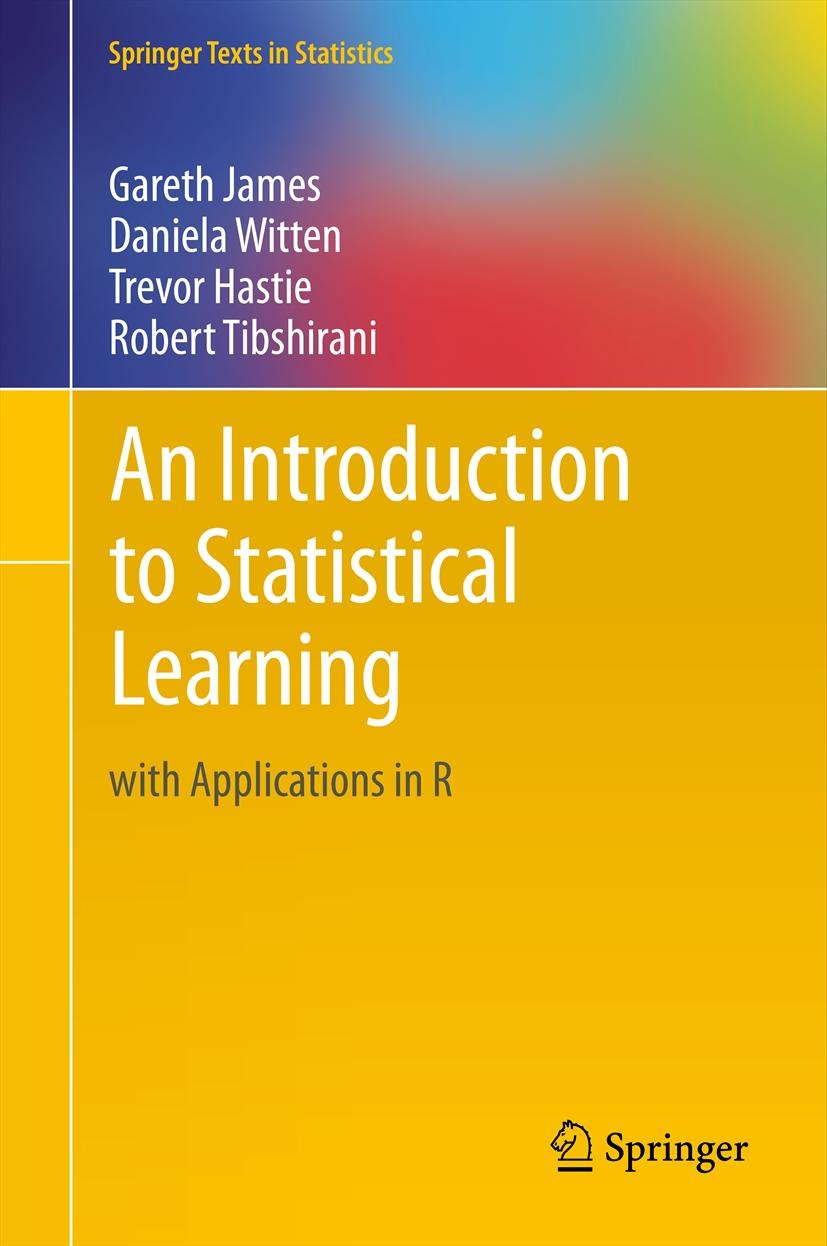
\includegraphics[width=0.6\textwidth]{intro/isl_cover}}
			\end{center}
			\begin{center}
				\href{www.statlearning.com}{\bfseries\blue ISLR}
			\end{center}
		\end{column}
	\end{columns}
	\bottomline{We will add to the content and be slightly more mathematical.}
\end{frame}

\begin{frame}{Literature: The more in-depth Tome}
	\begin{columns}
		\begin{column}{0.6\textwidth}
			\begin{itemize}
				\item This is a well-known reference text by two of the co-authors of ISLR.
				\item It also is freely available as a
					\href{https://web.stanford.edu/~hastie/ElemStatLearn/printings/ESLII_print12.pdf}{\blue\underline{PDF}}.
				\item This is the \href{https://web.stanford.edu/~hastie/ElemStatLearn/}{\blue\underline{book's website}}.
				\item The book covers more topics than ISLR and provides a more formal background. 
				\item We'll use some data sets from this book that are not used in ISLR.
			\end{itemize}
		\end{column}
		\begin{column}{0.4\textwidth}
			\begin{center}
				\href{https://web.stanford.edu/~hastie/ElemStatLearn/}{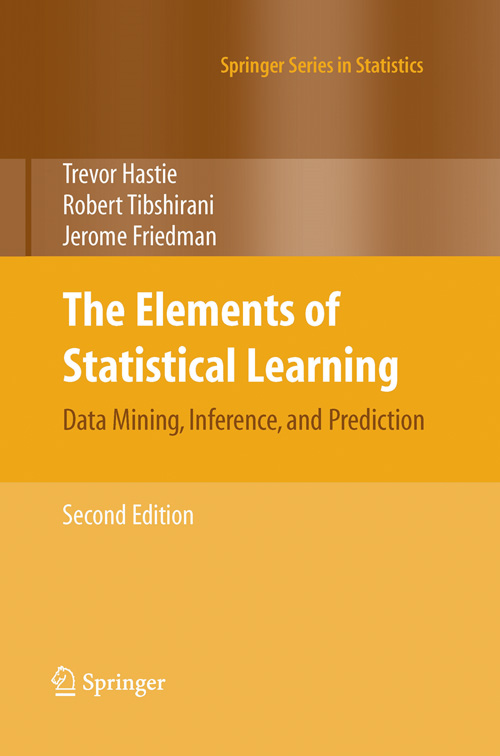
\includegraphics[width=0.6\textwidth]{intro/esl_cover}}
			\end{center}
			\begin{center}
				\href{https://web.stanford.edu/~hastie/ElemStatLearn/}{\bfseries\blue ESL}
			\end{center}
		\end{column}
	\end{columns}
	\bottomline{Consider this a reference for concepts in ISLR.}
\end{frame}

\begin{frame}{Literature: Foundations}
	\begin{columns}
		\begin{column}{0.6\textwidth}
			\begin{itemize}
				\item An excellent introduction to statistics, deriving everything from Bayesian probabilities.
				\item We won't cover this book, but refer to it to lay some foundations.
				\item Develops the theory around examples.
				\item Explains well why things are done the way they are.
			\end{itemize}
		\end{column}
		\begin{column}{0.4\textwidth}
			\begin{center}
				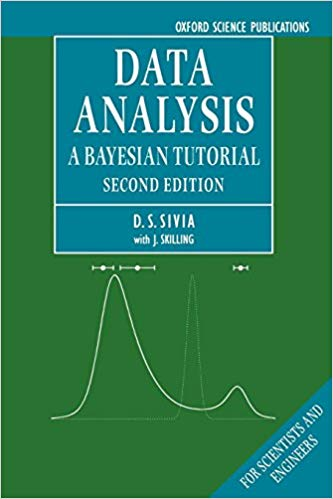
\includegraphics[width=0.6\textwidth]{intro/abt2_cover}
			\end{center}
			\begin{center}
				{\bfseries\blue ABT}
			\end{center}
		\end{column}
	\end{columns}
	\bottomline{Highly recommended!}
\end{frame}

\begin{frame}{What is Statistical Learning?}
	\begin{itemize}
		\item Statistical learning refers to various tools and methods for \emph{understanding} data.
		\item We usually distinguish between \emph{supervised} and \emph{unsupervised} methods.
		\item Supervised methods try to predict \emph{outputs} from \emph{inputs}.
		\item Unsupervised methods try to find \emph{structures} in the \emph{inputs}.
		\item We illustrate this briefly with some data sets.
	\end{itemize}
	\bottomline{The next lecture will cover this in more detail.}
\end{frame}

\begin{frame}{But what about Machine Learning?}
	\begin{Quote}%
		{Machine learning (ML) is the scientific study of algorithms and
		statistical models that computer systems use to perform a specific task
		without using explicit instructions, relying on patterns and inference
		instead. It is seen as a subset of artificial intelligence.}%
		{\href{https://en.wikipedia.org/wiki/Machine_learning}{Wikipedia page on Machine Learning}}
	\end{Quote}
	\begin{Quote}%
		{"Statistical learning" redirects here.}%
		{\href{https://en.wikipedia.org/wiki/Machine_learning}{Wikipedia page on Machine Learning}}
	\end{Quote}
	\bottomline{Machine Learning is just a fancy new name. It sure sounds cool!}	
\end{frame}

\begin{frame}{Wage Data}
	\begin{itemize}
		\item Here we refer to the \dat{Wage} data set.
		\item The \dat{Wage} data set contains data related to a group of males from the US.
		\item We are interested in how \dat{age}, \dat{education} and
			calendar \dat{year} affect \dat{wage}.
		\item We are going to \emph{visualize} the data to get a first understanding\\
			of the relationships among the variables.
	\end{itemize}
	\bottomline{Note the notation for data sets and variables.}
\end{frame}

\begin{frame}{Wage Data}
	\vspace{-1cm}
	\begin{center}
		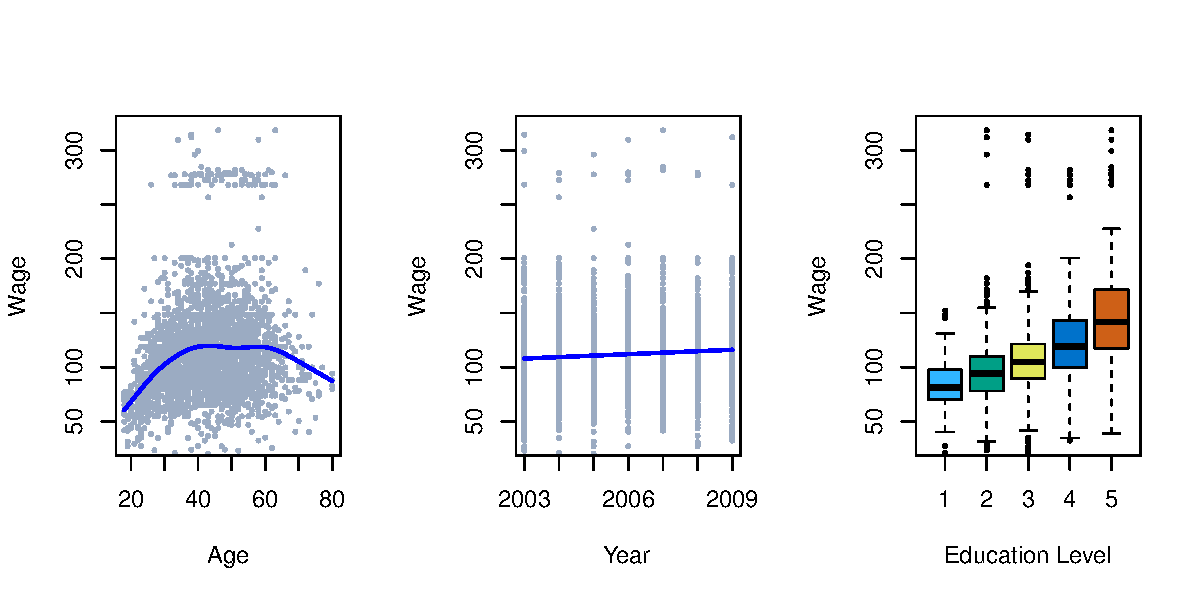
\includegraphics[width=0.7\textwidth]{1_1}
	\end{center}
	\vspace{-5mm}
	\begin{itemize}
		\item There is a correlation between \dat{age} and the average \dat{wage}.
		\item There is a slow but steady increase of \dat{wage} over time.
		\item The \dat{education} clearly has an impact on the \dat{wage}.
	\end{itemize}
	\bottomline{Visualization is extremely important. Always have a look first!}
\end{frame}

\begin{frame}{Stock Market Data}
	\begin{center}
		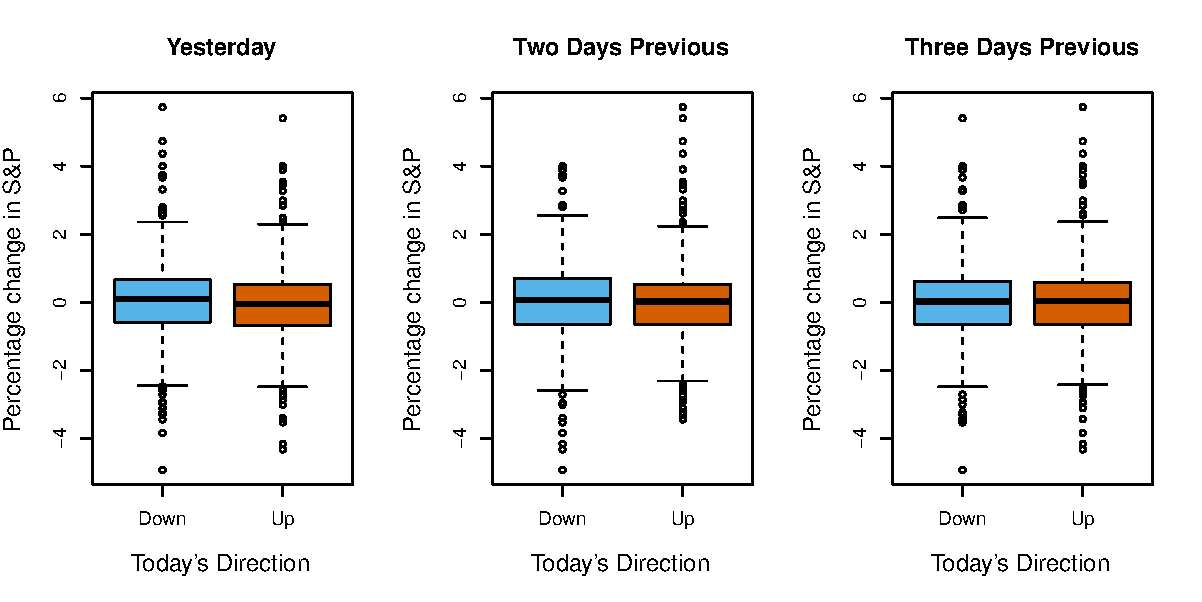
\includegraphics[width=0.7\textwidth]{1_2}

		{\footnotesize We would like to predict today's market direction from what happened
		in the previous days.}
	\end{center}
	\bottomline{We can not stress enough the importance of visualization.}
\end{frame}

\begin{frame}{Stock Market Data}
	\begin{columns}
		\begin{column}{0.6\textwidth}
			\begin{itemize}
				\item The \dat{Wage} data set involved \emph{quantitative} data.
				\item This is referred to as a \emph{regression} problem.
				\item Other problems involve predicting \emph{qualitative} data.
				\item These are \emph{classification} problems.
				\item For example, predicting whether the stock market goes up or down.
				\item The \dat{Smarket} data set provides daily percentage returns for
					S\&P 500 over five years.
			\end{itemize}
		\end{column}
		\begin{column}{0.4\textwidth}
			\vspace{-1.2cm}
			\begin{center}
				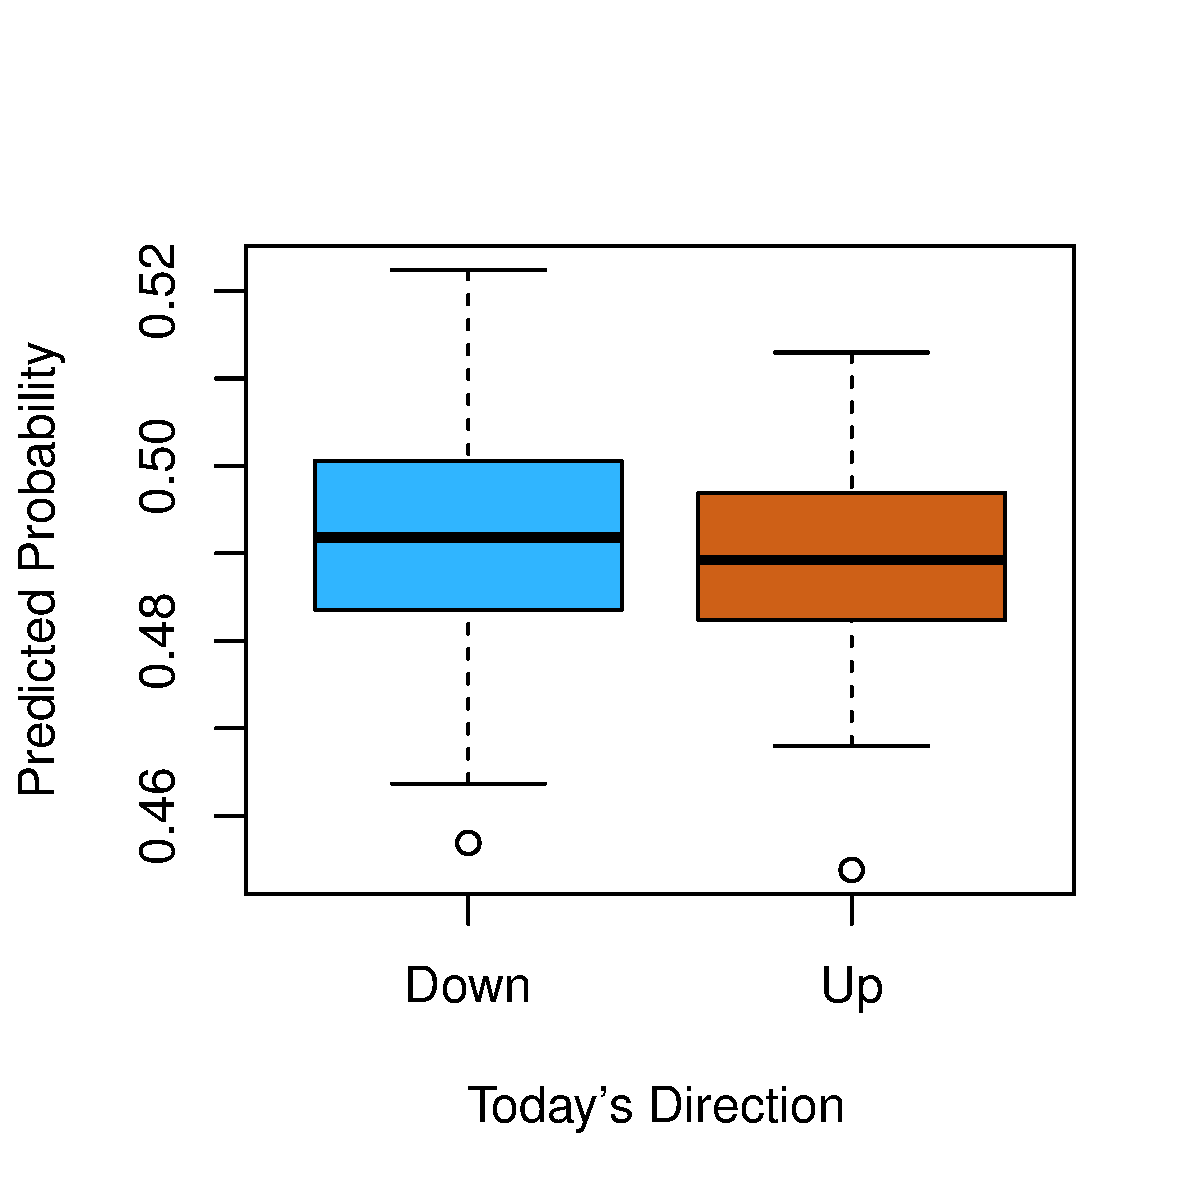
\includegraphics[width=0.98\textwidth]{1_3}

				\begin{minipage}[b]{0.7\textwidth}
					{\footnotesize Correct prediction 60\% of the time using quadratic discriminant analysis.}
				\end{minipage}
			\end{center}
		\end{column}
	\end{columns}
	\bottomline{Obviously, there is a lot of interest in this kind of problem.}
\end{frame}

\begin{frame}{Gene Expression Data}
	\vspace{-3mm}
	\begin{center}
		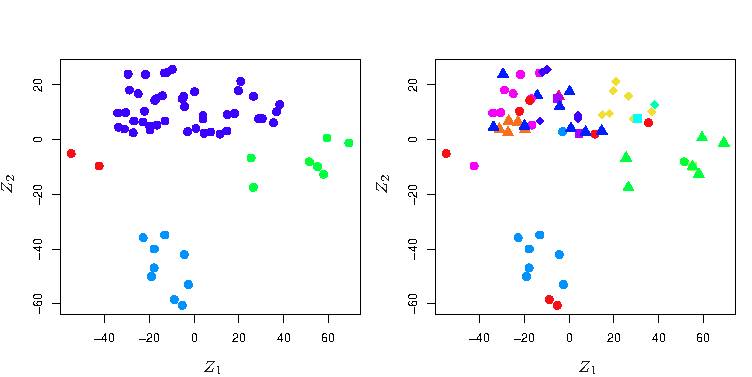
\includegraphics[width=0.54\textwidth]{1_4}
	\end{center}
	\vspace{-3mm}
	\begin{itemize}
		\item The \dat{NCI60} dataset contains 6,830 gene expression measurements \\
			for 64 cell lines of 14 different cancer types.
		\item The figure shows scatter plots of the first two \emph{principal components}, $Z_1$ and $Z_2$. 
		\item Cell lines of the same cancer type tend to cluster in $\{Z_1, Z_2\}$ space.
	\end{itemize}
	\bottomline{This is an example of \emph{unsupervised} learning.}
\end{frame}

\begin{frame}{Some Nomenclature}
	\begin{itemize}
		\item In most scenarios (certainly in all \emph{supervised} scenarios) there are two types of data:
			\begin{itemize}
				\item The data we consider the description of a situation.
				\item The data we consider the outcome of a situation.
			\end{itemize}
		\item The former are called \emph{input variables}, \emph{predictors}, \emph{independent variables}, \\
			\emph{features} or simply \emph{variables}.\\
			For example, in the \dat{Wage} data set these are \dat{age}, \dat{year}, \dat{education} and so on.
		\item The latter are called \emph{output variables}, \emph{dependent variables} or \emph{responses}.\\
			For example, in the \dat{Wage} data set it would be \dat{wage}.
	\end{itemize}
	\bottomline{We'll use the various terms interchangeably but stay true to the concepts.}
\end{frame}

\begin{frame}{Beware of Causality Claims}
	\begin{columns}
		\begin{column}{0.6\textwidth}
			\begin{itemize}
				\item The distinction between predictors and responses seems to imply a causal connection.  
				\item This is in general \emph{not} the case!
				\item Be \emph{very} careful about this!
				\item It is possible, however, to formalize the establishment of causal connections.
				\item The book on the right is the seminal work\\ on this subject.
				\item Formalizing causality is far beyond the scope\\ of this course.
			\end{itemize}
		\end{column}
		\begin{column}{0.4\textwidth}
			\begin{center}
				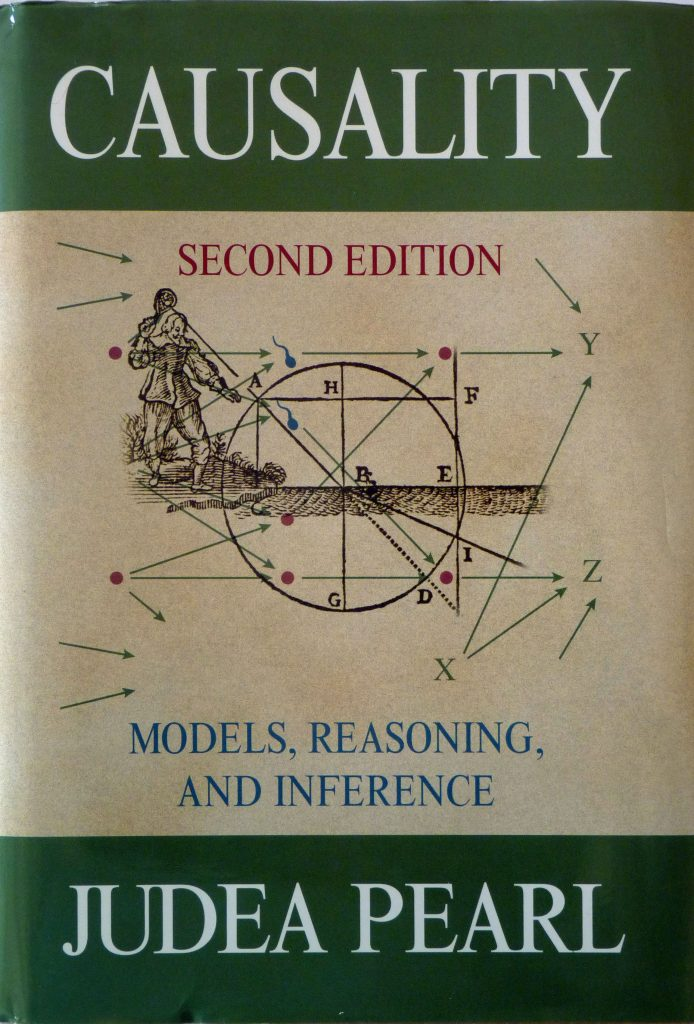
\includegraphics[width=0.6\textwidth]{intro/caus_cover}
			\end{center}
			\begin{center}
				{\bfseries\blue CAUS}
			\end{center}
		\end{column}
	\end{columns}
	\bottomline{Don't make formal claims of causality without reading (at least part of) this book.}
\end{frame}

\begin{frame}{Course Premises}
	\begin{center}
		\begin{minipage}[t]{0.8\textwidth}
			\begin{itemize}
				\item Many statistical learning methods are relevant in a wide range of disciplines.
				\item Statistical Learning should not be viewed as a series of black boxes.
				\item While it is important to understand the methods, their technical implementation 
					is (mostly) not our concern.
				\item We presume you are interested in applying statistical learning to real world problems.
			\end{itemize}
		\end{minipage}
	\end{center}
	\bottomline{We will be more mathematically inclined than the ISLR book. You can take it.}
\end{frame}

\begin{frame}{Course Outline}
	\begin{columns}
		\begin{column}{0.5\textwidth}
			\begin{enumerate}
				\item Introduction
				\item Statistical Learning
				\item Linear Regression
				\item Classification
				\item Resampling Methods
				\item Model Selection \& Regularization
			\end{enumerate}
		\end{column}
		\begin{column}{0.5\textwidth}
			\begin{enumerate}
					\setcounter{enumi}{6}
				\item Beyond Linearity
				\item Tree-Based Methods
				\item Support Vector Machines
				\item Unsupervised Learning
				\item Neural Networks \& Deep Learning
				\item Reinforcement Learning
			\end{enumerate}
		\end{column}
	\end{columns}
	\bottomline{This is the ISLR book content plus neural networks and reinforcement learning.}
\end{frame}

\begin{frame}{Notation: Feature Matrix}
	\begin{itemize}
		\item The predictors of a data set with $p$ predictors and $n$ observations\\
			are represented as a matrix like this:
	\end{itemize}
	\vspace{-8mm}
	\begin{center}
		\[ \bm{X} = 
			\begin{pmatrix}
				x_{11} & x_{12} & \dots & x_{1p} \\ 
				x_{21} & x_{22} & \dots & x_{2p} \\ 
				\vdots & \vdots & \ddots & \vdots \\
				x_{n1} & x_{n2} & \dots & x_{np} \\ 
			\end{pmatrix}
		\]
	\end{center}
	\begin{itemize}
		\item Each \emph{row} represents one observation of all variables.
		\item Each \emph{column} represents all observations of one variable.
	\end{itemize}
	\bottomline{Notation is hard to get right and boring. Please bear with us.}
\end{frame}

\begin{frame}{Notation: Feature Rows \& Columns}
	\vspace{-3mm}
	\begin{columns}[t]
		\begin{column}{0.5\textwidth}
			\begin{itemize}
				\item We might be interested the rows of $\bm{X}$.
				\item We write the rows as $x_1, x_2, \dots, x_n$.
				\item Each $x_i$ is a \emph{vector} of length $p$. 
				\item For the \dat{Wage} data set the components of the $x_i$
					would be \dat{age}, \dat{education}, \dat{year} and so on.
			\end{itemize}
			\vspace{-12mm}
			\begin{center}
				\[
					x_i =
					\begin{pmatrix}
						x_{i1} \\
						x_{i2} \\
						\vdots \\
						x_{ip} \\
					\end{pmatrix}
				\]
			\end{center}
		\end{column}
		\begin{column}{0.5\textwidth}
			\begin{itemize}
				\item Or we need to refer to the columns of $\bm{X}$.
				\item We write the columns as $\bm{x}_1, \bm{x}_2, \dots, \bm{x}_p$.
				\item Each $\bm{x}_j$ is a \emph{vector} of length $n$. 
			\end{itemize}
			\vspace{2mm}
			\begin{center}
				\[
					\bm{x}_j =
					\begin{pmatrix}
						\bm{x}_{1j} \\
						\bm{x}_{2j} \\
						\vdots \\
						\bm{x}_{nj} \\
					\end{pmatrix}
				\]
			\end{center}
		\end{column}
	\end{columns}
	\bottomline{Note that we represent vectors as \emph{column vectors} by default.}
\end{frame}

\begin{frame}{Notation: Transposition}
	\vspace{-3mm}
	\begin{columns}[t]
		\begin{column}{0.5\textwidth}
			\begin{itemize}
				\item Now $\bm{X}$ can be written like this:
			\end{itemize}
			\vspace{-5mm}
			\begin{center}
				\[
					\bm{X} =
					\begin{pmatrix}
						\bm{x}_1 & \bm{x}_2 & \dots & \bm{x}_p \\
					\end{pmatrix}
				\]
			\end{center}
			\begin{itemize}
				\item Or like this:
			\end{itemize}
			\vspace{-9mm}
			\begin{center}
				\[
					\bm{X} =
					\begin{pmatrix}
						x_1^T \\ x_2^T \\ \vdots \\ x_n^T \\
					\end{pmatrix}
				\]
			\end{center}
		\end{column}
		\begin{column}{0.5\textwidth}
			\begin{itemize}
				\item The ${}^T$ denotes the \emph{transpose} of a matrix:
			\end{itemize}
			\vspace{-9mm}
			\begin{center}
				\[
					\bm{X}^T =
					\begin{pmatrix}
						x_{11} & x_{21} & \dots & x_{n1} \\ 
						x_{12} & x_{22} & \dots & x_{n2} \\ 
						\vdots & \vdots & \ddots & \vdots \\
						x_{1p} & x_{2p} & \dots & x_{np} \\ 
					\end{pmatrix}
				\]
			\end{center}
			\begin{itemize}
				\item Or of a vector:
			\end{itemize}
			\vspace{-9mm}
			\begin{center}
				\[
					x_i^T =
					\begin{pmatrix}
						x_{i1} & x_{i2} & \dots & x_{ip} \\
					\end{pmatrix}
				\]
			\end{center}
		\end{column}
	\end{columns}
	\bottomline{Being consistent about transposition is important.}
\end{frame}

\begin{frame}{Notation: Response Vector}
	\vspace{-3mm}
	\begin{columns}[t]
		\begin{column}{0.5\textwidth}
			\begin{itemize}
				\item We write the $i$th observation of a response, say \dat{wage}, as $y_i$.
				\item The set of all $n$ observations is then the vector 
			\end{itemize}
			\vspace{-8mm}
			\begin{center}
				\[
					\bm{y} =
					\begin{pmatrix}
						y_1 \\ y_2 \\ \vdots \\ y_n \\
					\end{pmatrix}
				\]
			\end{center}
		\end{column}
		\begin{column}{0.5\textwidth}
			\begin{itemize}
				\item In general, we write vectors of length $n$ in {\bfseries bold} face:
			\end{itemize}
			\vspace{-9mm}
			\begin{center}
				\[
					\bm{a} =
					\begin{pmatrix}
						a_1 \\ a_2 \\ \vdots \\ a_n \\
					\end{pmatrix}
				\]
			\end{center}
			\begin{itemize}
				\item However, vectors of different lengths, for example $p$, are written in
					normal face:
			\end{itemize}
			\vspace{-9mm}
			\begin{center}
				\[ x_i \]
			\end{center}
		\end{column}
	\end{columns}
	\bottomline{This convention is purely for notational clarity \& convenience.}
\end{frame}

\begin{frame}{Notation: Summary}
	\begin{popblock}{0.6\textwidth}{With $n$ observations in a data set with $p$ features:}
		\begin{tabular}[h]{lcc}
			{\bfseries\blue object} & {\bfseries\blue space} & {\bfseries\blue notation} \\
			scalar & $\R$ & $a$ \\
			column vector ($k = n$)  & $\R^{n \times 1}$ or $\R^n$ & $\bm{a}$ \\
			row vector ($k = n$)  & $\R^{1 \times n}$ or $\R^n$ & $\bm{a}^T$ \\
			column vector ($k \ne n$)  & $\R^{k \times 1}$ or $\R^k$ & $a$ \\
			row vector ($k \ne n$)  & $\R^{1 \times k}$ or $\R^k$ & $a^T$ \\
			matrix ($r$ rows, $d$ columns) & $\R^{r\times d}$ & $\bm{A}$ \\
			\hline
			feature matrix & $\R^{n\times p}$ & $\bm{X}$ \\
			$i$th feature row & $\R^{1\times p}$ or $\R^p$ & $x_i^T$ \\
			$j$th feature column & $\R^{n\times 1}$ or $\R^n$ & $\bm{x}_j$ \\
			response vector & $\R^{n\times 1}$ or $\R^n$ & $\bm{y}$ \\
		\end{tabular}
	\end{popblock}
	\bottomline{Forgive us for occasionally relaxing some of this in hand writing.}
\end{frame}

\begin{frame}{Symbol Manipulation: Matrix Multiplication}
	\begin{itemize}
		\item For two matrices $\bm{A} \in \R^{r\times d}$ and $\bm{B} \in \R^{d\times s}$ their \emph{matrix product}
			$\bm{C} \in \R^{r\times s}$ is:
	\end{itemize}
	\vspace{-12mm}
	\begin{center}
		\[ \bm{C} = \bm{AB} \]
	\end{center}
	\begin{itemize}
		\item The \emph{components} $c_{ij} = (\bm{C})_{ij} = (\bm{AB})_{ij}$ are computed as follows: 
	\end{itemize}
	\vspace{-12mm}
	\begin{center}
		\[ c_{ij} = \sum_{k = 1}^{d} a_{ik}b_{kj} \]
	\end{center}
	\vspace{-5mm}
	\begin{itemize}
		\item For example:
	\end{itemize}
	\vspace{-12mm}
	\begin{center}
		\[
			\bm{AB} =
			\begin{pmatrix}
				1 & 2 \\ 3 & 4 \\
			\end{pmatrix}
			\begin{pmatrix}
				5 & 6 \\ 7 & 8 \\
			\end{pmatrix}
			=
			\begin{pmatrix}
				1\times 5 + 2\times 7 & 1\times 6 + 2\times 8\\ 
				3\times 5 + 4\times 7 & 3\times 6 + 4\times 8 \\
			\end{pmatrix}
			=
			\begin{pmatrix}
				19 & 22 \\ 43 & 50 \\
			\end{pmatrix}
		\]
	\end{center}
	\bottomline{The ISLR book is a bit shy about using this. We are not.}
\end{frame}

\begin{frame}{Symbol Manipulation: Useful Properties}
	\vspace{-5mm}
	\begin{columns}[t]
		\begin{column}{0.5\textwidth}
			\begin{itemize}
				\item Matrix multiplication is \emph{not} commutative:
					\[ \bm{AB} \ne \bm{BA} \]
				\item Matrix multiplication is associative:
					\[ \bm{CBA} = \bm{C}(\bm{BA}) = (\bm{CB})\bm{A} \]
			\end{itemize}
		\end{column}
		\begin{column}{0.5\textwidth}
			\begin{itemize}
				\item Matrix multiplication is distributive:
					\[ \bm{C} (\bm{B} + \bm{A}) = \bm{CB} + \bm{CA} \]
				\item The transpose of a matrix product is:
					\[ (\bm{BA})^T = \bm{A}^T\bm{B}^T \]
			\end{itemize}
		\end{column}
	\end{columns}
	\vspace{-2mm}
	\bottomline{We left out a few ``obvious'' properties.}
\end{frame}

\begin{frame}{Symbol Manipulation: Matrix Inversion}
	\vspace{-2mm}
	\begin{columns}[t]
		\begin{column}{0.8\textwidth}
			\begin{itemize}
				\item A \emph{square matrix} $\bm{A} \in \R^{d\times d}$ is \emph{invertible} if, 
					and only if, $\exists\bm{A}^{-1}$ such that:
					\[ \bm{A}\bm{A}^{-1} = \bm{A}^{-1}\bm{A} = \bm{I} \]
				\item Where the components of the  \emph{unit matrix} $\bm{I} \in \R^{d\times d}$ are:
					\[ (\bm{I})_{ij} = \delta_{ij} = 
						\begin{cases}
							1 & i = j \\
							0 & i \ne j \\
						\end{cases}
					\]
					\[ \implies \bm{I}\bm{M} = \bm{M}, \bm{M} \in \R^{d\times s} \]
				\item Furthermore:
					\[ \exists\bm{A}^{-1}\implies\exists(\bm{A}^T)^{-1} = (\bm{A}^{-1})^T\]
			\end{itemize}
		\end{column}
	\end{columns}
	\bottomline{Inverting matrices can be hard -- we'll leave that to the computer.}
\end{frame}

\begin{frame}{Symbol Manipulation: Gradients}
	\begin{columns}[t]
		\begin{column}{0.5\textwidth}
			\begin{itemize}
				\item The \emph{gradient} of a \emph{scalar function} $f(a) \in \R$ wrt.\ a vector $a \in \R^k$ is
					a \emph{column vector} of dimension $k$ with components ${\partial f}/{\partial a_i}$: 
			\end{itemize}
			\vspace{-5mm}
			\begin{center}
				\[ 
					\frac{\partial f}{\partial a} = \nabla_a\, f =
					\begin{pmatrix}
						{\partial f}/{\partial a_1} \\ 
						{\partial f}/{\partial a_2} \\
						\vdots \\
						{\partial f}/{\partial a_k} \\ 
					\end{pmatrix}
				\]
			\end{center}
		\end{column}
		\begin{column}{0.5\textwidth}
			\begin{itemize}
				\item In particular, the gradient wrt.\ the vector $a$ of the \emph{scalar product} $a^T b = b^T a$ is:
			\end{itemize}
			\begin{center}
				\[ 
					\nabla_a\, a^T b = \nabla_a\, b^T a = b =
					\begin{pmatrix}
						b_1 \\ b_2 \\ \vdots \\ b_k \\
					\end{pmatrix}
				\]
			\end{center}
		\end{column}
	\end{columns}
	\bottomline{This is by no means obvious, but we can't dive deeply into differential geometry here.}
\end{frame}

\begin{frame}{The Gradient Illustrated}
	\begin{center}
		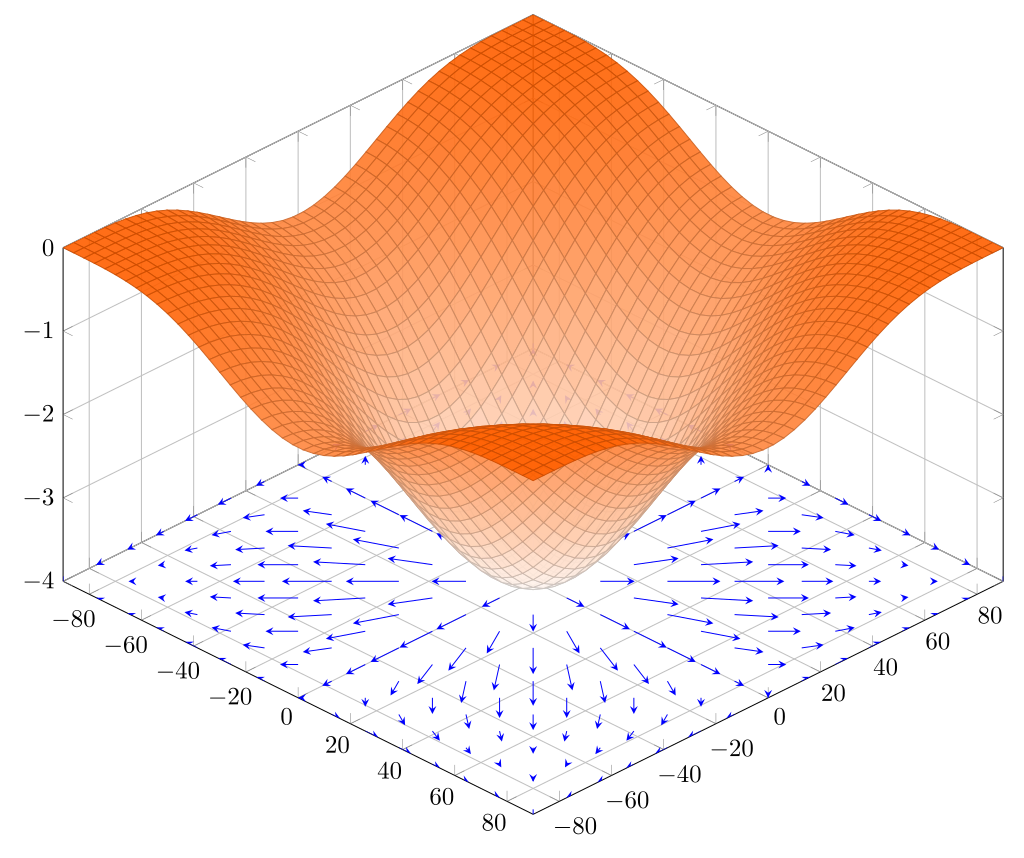
\includegraphics[width=0.5\textwidth]{intro/gradient}
		{\antsize \[ f(x, y) = - (\cos^2 x + \cos^2 y)^2 \]}
	\end{center}
	\bottomline{Think of the gradient as the direction and magnitude of the steepest ascent.}
\end{frame}

\begin{frame}{The Work Environment}
	\begin{columns}
		\begin{column}{0.6\textwidth}
			\begin{itemize}
				\item We'll use Python and a number of common libraries
					for the labs and exercises.
				\item For interactive work (most labs and exercises) we'll use
					jupyter notebooks.
				\item We have prepared a Python library ({\tt islpy}) that provides
					easy access to \& documentation for all the data sets.
				\item We provide a virtual machine running Xubuntu 18.04 with everything
					pre-installed.
			\end{itemize}
		\end{column}
		\begin{column}{0.4\textwidth}
			\begin{center}
				\href{https://www.python.org/}{
\includegraphics[width=0.6\textwidth]{intro/python-logo}}
			\end{center}
			\begin{center}
				\href{https://numpy.org/}{
\includegraphics[width=0.6\textwidth]{intro/numpy_logo}}
			\end{center}
			\begin{center}
				\href{https://jupyter.org/}{
\includegraphics[width=0.2\textwidth]{intro/jupyter_logo}}
			\end{center}
			\begin{center}
				\href{https://xubuntu.org/}{
\includegraphics[width=0.6\textwidth]{intro/xubuntu_logo}}
			\end{center}
		\end{column}
	\end{columns}
	\bottomline{There is not enough room for the logos of all the libraries!}	
\end{frame}

\begin{frame}{The Virtual Machine}
	\begin{center}
		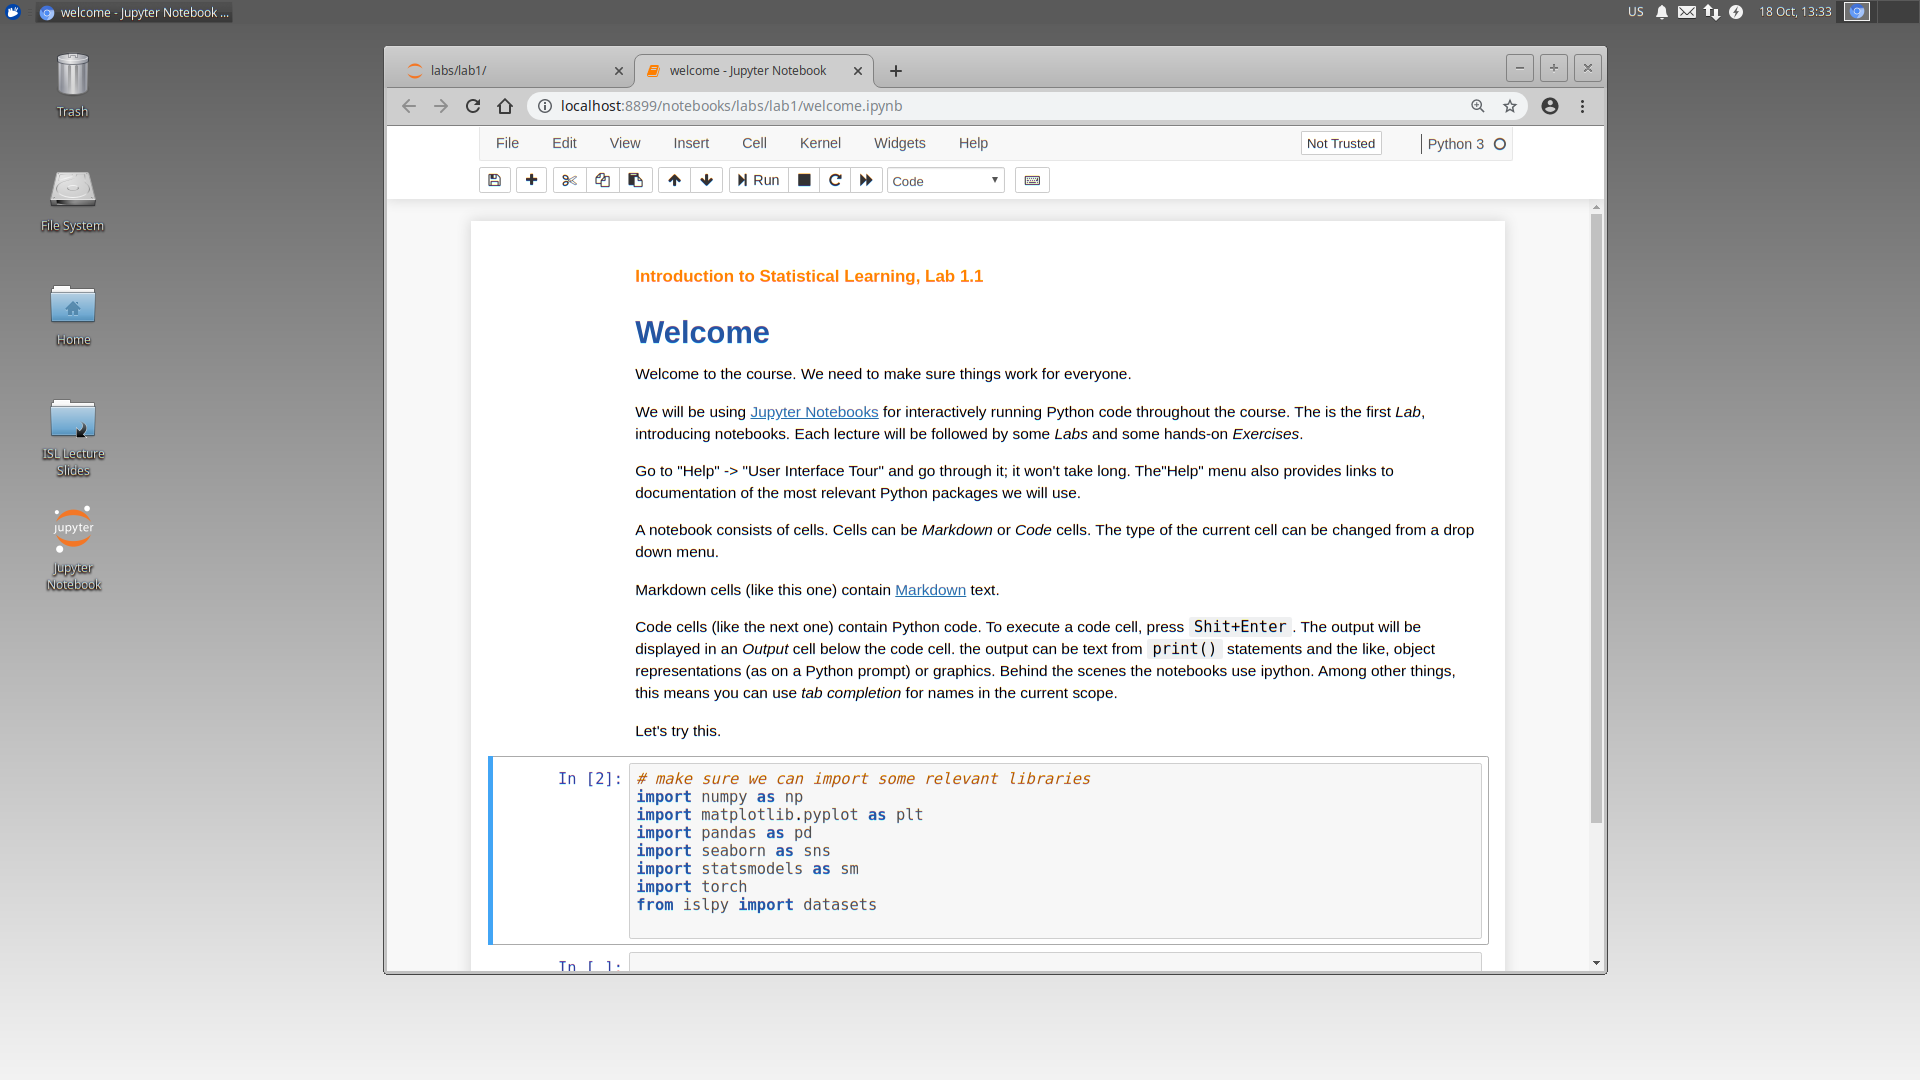
\includegraphics[width=0.7\textwidth]{intro/isl_vm_desktop}
	\end{center}
	\bottomline{Let's make sure this works for everyone.}
\end{frame}

\end{document}
